%----------------------------------------------------------------------------------------
%	Paquetes y configuración
%----------------------------------------------------------------------------------------
\documentclass{article}

\usepackage[utf8]{inputenc}
\usepackage[spanish,es-lcroman]{babel}
\usepackage{fancyhdr}
\usepackage{lastpage}
\usepackage{extramarks}
\usepackage[usenames,dvipsnames]{color}
\usepackage{graphicx}
\usepackage{listings}
\usepackage{xparse}
\usepackage{courier}
\usepackage{amsmath}
\usepackage{enumitem}
\usepackage{hyperref}
\usepackage{mathtools}
\usepackage{lipsum}
\usepackage{float}
\usepackage{algorithm}
\usepackage{algpseudocode}
\usepackage{booktabs}
\floatplacement{figure}{H}


% Margenes
\topmargin=-0.45in
\evensidemargin=0in
\oddsidemargin=0in
\textwidth=6.5in
\textheight=9.0in
\headsep=0.25in

\renewcommand{\arraystretch}{1.2}

% Header y footer
\pagestyle{fancy}
\lhead{}
\chead{\tareaRamo\ (\tareaProfesor): \tareaTitulo} % Centro
\rhead{\firstxmark}
\lfoot{UTFSM CSJ - Departamento de Informática}
\cfoot{}
\rfoot{Página\ \thepage\ de\ \protect\pageref{LastPage}} % Pagina
\renewcommand\headrulewidth{0.4pt}
\renewcommand\footrulewidth{0.4pt}

\setlength\parindent{0pt} % Eliminar la indentación

%----------------------------------------------------------------------------------------
%	Inclusión de python con systax highlight
%----------------------------------------------------------------------------------------
\renewcommand\lstlistingname{Script}
\renewcommand\lstlistlistingname{Scripts}

\definecolor{MyDarkGreen}{rgb}{0.0,0.4,0.0}
\lstloadlanguages{Python}
\lstset{
  language=Python,
  frame=single, % Single frame around code
  basicstyle=\small\ttfamily, % Use small true type font
  keywordstyle=[1]\color{BlueViolet}\bf, % Function names
  keywordstyle=[2]\color{Purple}, % Arguments
  keywordstyle=[3]\color{Blue}\underbar,
  identifierstyle=,
  commentstyle=\usefont{T1}{pcr}{m}{sl}\color{MyDarkGreen}\small,
  stringstyle=\color{Purple},
  showstringspaces=false,
  tabsize=5,
  morekeywords={rand,},
  morekeywords=[2]{on, off, interp},
  morekeywords=[3]{y, range},
  morecomment=[l][\color{Blue}]{...},
  numbers=left,
  firstnumber=1,
  numberstyle=\tiny\color{Gray},
  stepnumber=1
}

\newcommand{\python}[2]{
  \begin{itemize}
    \item[]\lstinputlisting[language=Python,caption=#2,label=#1]{#1.py}
  \end{itemize}
}

%----------------------------------------------------------------------------------------
%	Meta Información
%----------------------------------------------------------------------------------------
\newcommand{\tareaTitulo}{Tarea\ 1}
\newcommand{\tareaFecha}{\today}
\newcommand{\tareaRamo}{INF391 Reconocimiento\ de\ Patrones\ en\ Minería\ de\ Datos}
\newcommand{\tareaProfesor}{Marcelo\ Mendoza}

%----------------------------------------------------------------------------------------
%	Título
%----------------------------------------------------------------------------------------
\title{
  \Large\textmd{\textbf{\tareaRamo\\ \tareaTitulo}}\\
  \vspace{0.1in}
  \normalsize
  Universidad Técnica Federico Santa María, Campus San Joaquín\\
  Departamento de Informática\\
  \vspace{0.1in}
  \small{\textsc{\tareaFecha}}\\
  \vspace{0.1in}
  \large{\textsc{Profesor Marcelo Mendoza}}
  \vspace{1.5in}
}

\author{
    \textit{Juan Pablo Escalona} \\
    \small{juan.escalonag@alumnos.usm.cl} \\
    \small{201073515-k}
    \and
    \textit{Rafik Masad} \\
    \small{rafik.masad@alumnos.usm.cl} \\
    \small{201073519-2}
    \and
    \textit{Gianfranco Valentino}\\
    \small{gianfranco.valentino@alumnos.usm.cl}\\
    \small{2860574-9}
}
\date{}

%----------------------------------------------------------------------------------------
% Documento
%----------------------------------------------------------------------------------------
\begin{document}

\maketitle
\newpage

%----------------------------------------------------------------------------------------
% Índice
%----------------------------------------------------------------------------------------
% \setcounter{tocdepth}{3}
% \newpage
% \tableofcontents
% \newpage

%----------------------------------------------------------------------------------------
% Desarrollo
%----------------------------------------------------------------------------------------
\section*{Introducción}

En el presente informe se analizan los resultados obtenidos comparando diferentes técnicas de clustering sobre el dataset iris incluido en la librería \textit{sklearn}.

\section*{Análisis de los resultados obtenidos}
Se analizaron una gran diversidad de algoritmos, pero hay ciertos parámetros que son comunes entre ellos. Haciendo el símil con la teoría, tenemos que \emph{n\_clusters} corresponde a $K$, para ciertos
algoritmos que esperan dicho input. También existen diversas condiciones de termino, estas pueden considerarse como \emph{tol}, o tolerancia, es decir, cuanto es el máximo numero de cambios de puntos clasificados entre iteraciones
para terminar el algoritmo. Por ejemplo, 0.1 significa que si entre dos iteraciones consecutivas, el numero de puntos que cambiaron de cluster, es menor o igual que el 10\% del total de datos, se termina el algoritmo. Por otro lado, también
se limita el número máximo de iteraciones, ya que si bien, los métodos convergen a máximos locales, dependiendo del dataset y las semillas, podría tomar demasiadas iteraciones, aun cuando la solución es aceptable.

Para definir una medida común de errores, se intenta ver los labels originales, o bien, los que vienen con el dataset. Luego se comparan los grupos formados, con los esperados y se cuentan los puntos clasificados incorrectamente.

Ahora bien, lo último a tener en cuenta, es que los algoritmos que dependen de semillas, tienen resultados muy distintos dependiendo de estas, ya que al converger a máximos locales, el punto inicial es determinante, es por ello, que se realizan
multiples ejecuciones, y se mantiene el mejor resultado.

\newpage

\subsection*{1.1. \; K-means}

\begin{description}
  \item[Algoritmo:] K-means
  \item[Parámetros utilizados:] \hfill
    \begin{itemize}
      \item n\_clusters: 3
      \item tol: 0.1
      \item max\_iter: 300
      \item n\_jobs: 1
    \end{itemize}
  \item[Resultados]\hfill
    \begin{itemize}
      \item Errores: 14
      \item Accuracy:  90.7\%
      \item Tiempo de ejecución: 0.0123851 [s]
    \end{itemize}
\end{description}

\begin{figure}[H]
  \centering
  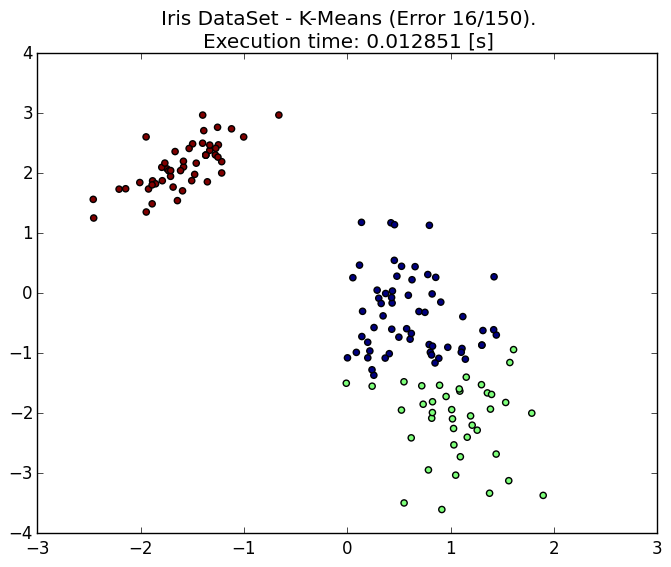
\includegraphics[width=0.666\textwidth]{img/K-Means.png}
  \caption{K-means++}
\end{figure}
\newpage



\subsection*{1.2. \; Minibatch K-means}
\begin{description}
  \item[Algoritmo:] Minibatch K-means
  \item[Parámetros utilizados:] \hfill
    \begin{itemize}
      \item n\_clusters: 3
      \item reassignment\_ratio: 0.01
      \item max\_iter: 100
      \item batch\_size: 5
      \item init: 'k-means++'
      \item n\_init: 3
      \item tol: 0.5
    \end{itemize}
  \item[Resultados]\hfill
    \begin{itemize}
      \item Errores: 15
      \item Accuracy:  90\%
      \item Tiempo de ejecución: 0.016015 [s]
    \end{itemize}
\end{description}

\begin{figure}[H]
  \centering
  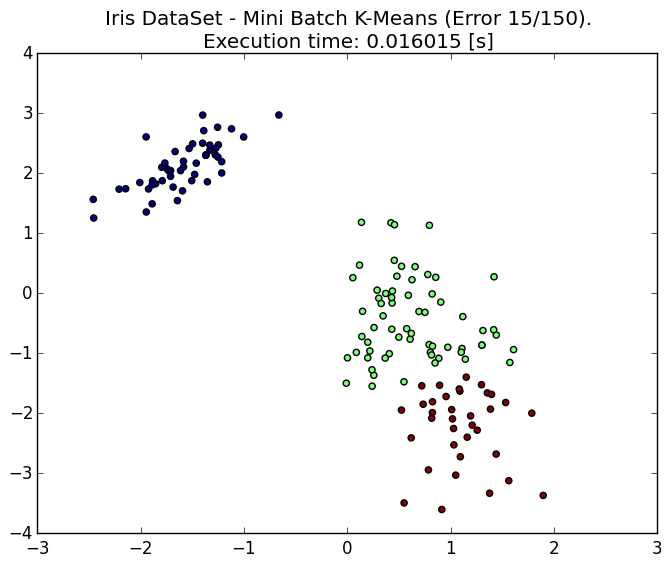
\includegraphics[width=0.666\textwidth]{img/MiniBatchK-Means.png}
  \caption{Minibatch k-means}
\end{figure}

En general k-means, al converger a un máximo local, es extremadamente dependiente de las semillas, explicando así las diferencias en la calidad de los resultados por ejecución.
\newpage



\subsection*{1.3. \; HAC}
\begin{description}
  \item[Algoritmo:] HAC
  \item[Parámetros utilizados:] \hfill
    \begin{itemize}
      \item n\_clusters: 3
      \item affinity: euclidean
      \item n\_components: None
      \item linkage: average
    \end{itemize}
  \item[Resultados]\hfill
    \begin{itemize}
      \item Errores: 16
      \item Accuracy:  89.3\%
      \item Tiempo de ejecución: 0.002657 [s]
    \end{itemize}
\end{description}

\begin{figure}[H]
  \centering
  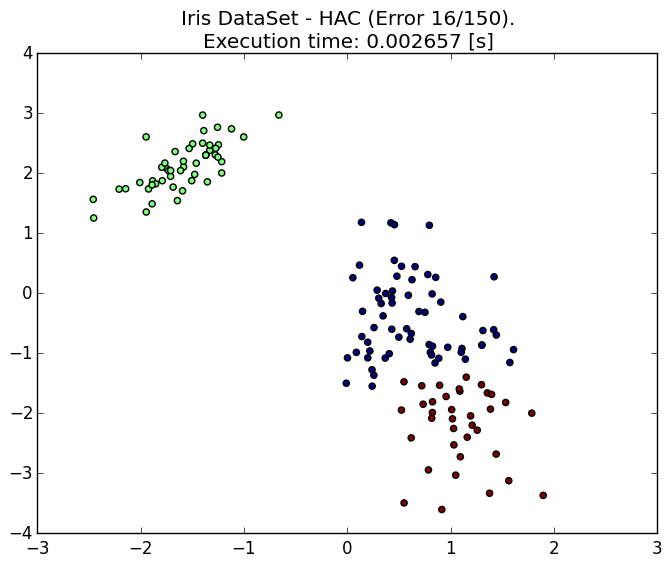
\includegraphics[width=0.666\textwidth]{img/HAC.png}
  \caption{HAC}
\end{figure}

\newpage




\subsection*{1.4. \; Ward}
\begin{description}
  \item[Algoritmo:] Ward
  \item[Parámetros utilizados:] \hfill
    \begin{itemize}
      \item n\_clusters: 3
    \end{itemize}
  \item[Resultados]\hfill
    \begin{itemize}
      \item Errores: 16
      \item Accuracy:  89.3\%
      \item Tiempo de ejecución: 0.011104 [s]
    \end{itemize}
\end{description}

\begin{figure}[H]
  \centering
  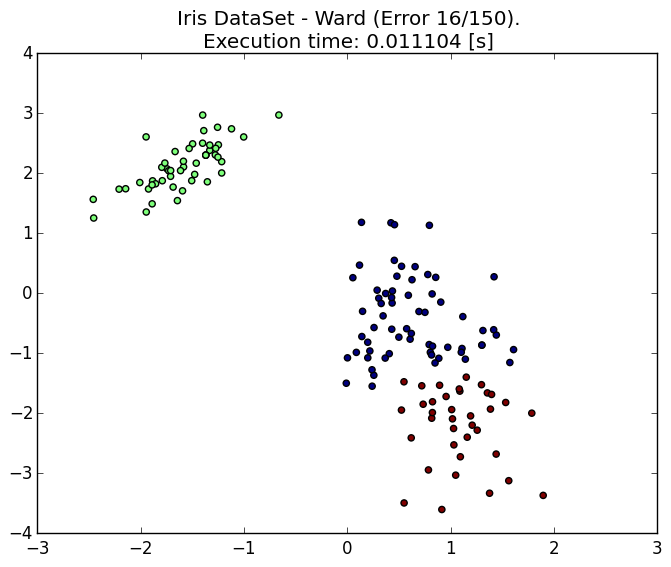
\includegraphics[width=0.666\textwidth]{img/Ward.png}
  \caption{Ward}
\end{figure}

\newpage




\subsection*{1.5. \; DBScan}

\begin{description}
  \item[Algoritmo:] DBScan
  \item[Parámetros utilizados:] \hfill
    \begin{itemize}
      \item min\_samples: 14
      \item eps: 0.5
    \end{itemize}
  \item[Resultados]\hfill
    \begin{itemize}
      \item Errores: 22
      \item Accuracy:  85.3\%
      \item Tiempo de ejecución: 0.031344 [s]
    \end{itemize}
\end{description}

\begin{figure}[H]
  \centering
  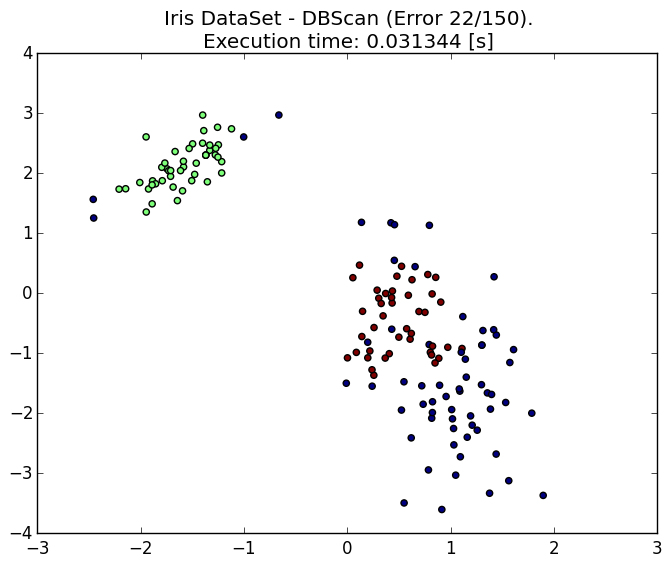
\includegraphics[width=0.666\textwidth]{img/DBScan.png}
  \caption{DBScan}
\end{figure}

\newpage





\subsection*{1.6. \; C-Means}

\begin{description}
  \item[Algoritmo:] C-Means
  \item[Parámetros utilizados:] \hfill
    \begin{itemize}
      \item c: 3
      \item m: 0.01
      \item error: 0.3
      \item maxiter: 20
      \item seed: None
    \end{itemize}
  \item[Resultados]\hfill
    \begin{itemize}
      \item Errores: 10-50\footnote{Muy variable}
      \item Accuracy:  60-90\%
      \item Tiempo de ejecución: 0.017491 [s]
    \end{itemize}
\end{description}

\begin{figure}[H]
  \centering
  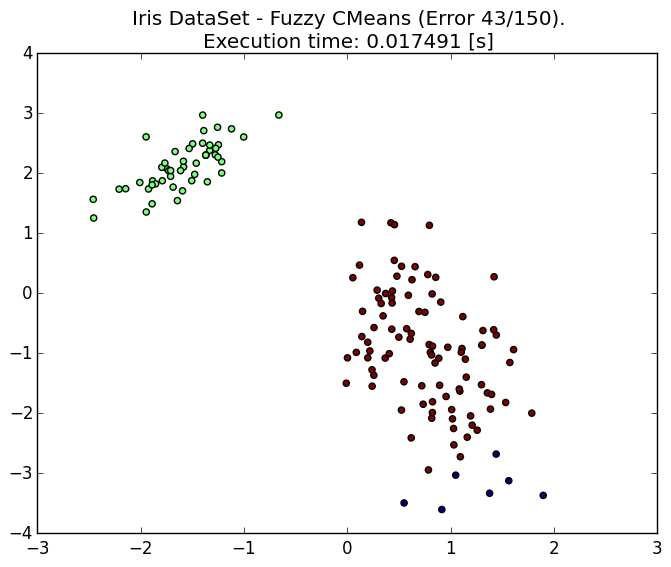
\includegraphics[width=0.666\textwidth]{img/FuzzyCMeans.png}
  \caption{C-Means}
\end{figure}

\newpage




\subsection*{1.7. \; Mean shift}

\begin{description}
  \item[Algoritmo:] Mean shift
  \item[Parámetros utilizados:] \hfill
    \begin{itemize}
      \item bandwidth: 0.9
      \item bin\_seeding: True
      \item min\_bin\_freq: 1
      \item cluster\_all: False
    \end{itemize}
  \item[Resultados]\hfill
    \begin{itemize}
      \item Errores: 33
      \item Accuracy:  78\%
      \item Tiempo de ejecución: 0.080781 [s]
    \end{itemize}
\end{description}

\begin{figure}[H]
  \centering
  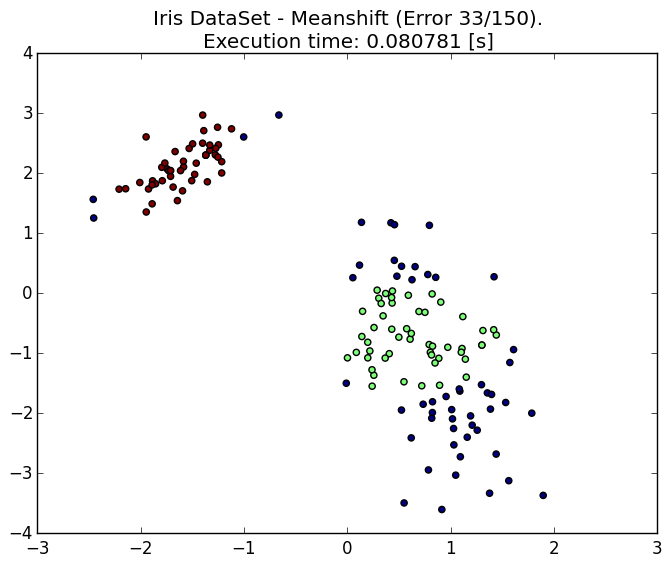
\includegraphics[width=0.666\textwidth]{img/Meanshift.png}
  \caption{Mean shift}
\end{figure}

\newpage




\subsection*{1.8. \; Spectral Clustering}

\begin{description}
  \item[Algoritmo:] Spectral Clustering
  \item[Parámetros utilizados:] \hfill
    \begin{itemize}
      \item n\_clusters: 3
      \item n\_components: 3
      \item eigen\_solver: ‘arpack’
      \item assign\_labels: ‘discretize’
      \item n\_init: 1
      \item weight: 9.5
    \end{itemize}
  \item[Resultados]\hfill
    \begin{itemize}
      \item Errores: 6
      \item Accuracy:  96\%
      \item Tiempo de ejecución: 0.064943 [s]
    \end{itemize}
\end{description}

\begin{figure}[H]
  \centering
  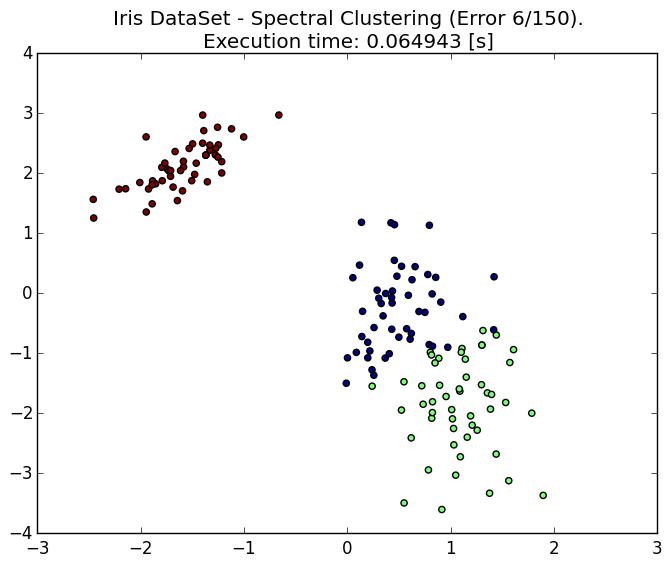
\includegraphics[width=0.666\textwidth]{img/SpectralClustering.png}
  \caption{Spectral Clustering}
\end{figure}

\newpage


\subsection*{2 \; Tabla comparativa}
En la siguiente tabla se resumen los errores y tiempos de cada algoritmo
\begin{center}
  \begin{tabular*}{0.666\textwidth}{@{\extracolsep{\fill}}l l l@{}}
      \midrule[1pt]
      Algoritmo & Errores & Tiempo [s] \\
      \midrule[0.4pt]
      Spectral Clustering  & 6     & 0.064943  \\
      k-means              & 14    & 0.012385  \\
      Minibatch k-means    & 15    & 0.016015  \\
      HAC                  & 16    & 0.002657  \\
      Ward                 & 16    & 0.011104  \\
      DBScan               & 22    & 0.031344  \\
      Mean shift           & 33    & 0.080781  \\
      C-Means              & 10-50 & 0.017491  \\
      \midrule[0.4pt]
  \end{tabular*}
\end{center}


\section*{Conclusiones}
En conclusion, podemos observar que el mejor resultado fue Spectral Clustering, y que los algoritmos que utilizan semillas, son muy dependientes de estas, por lo que se aplican técnicas como ejecuciones simultáneas con distintas semillas. Además, hay que recalcar el trade-off entre calidad y tiempo, si bien Spectral Clustering, tuvo el mejor resultado,  comparando con el resto de los algoritmos, en general tiende a demorarse entre 3 a 6 veces más aproximadamente. Y debemos tener en cuenta, que este dataset es de juguete, y que el comportamiento no necesariamente es el mismo al aumentar el número de K, y el número de datos, por lo que la técnica a utilizar debe considerar el comportamiento de los algoritmos frente a las distintas entradas, por lo que no habría un algoritmo único a utilizar frente a todos los casos.

% \section*{Referencias}

%   \begin{itemize}
%     \item ---
%   \end{itemize}

% \section*{Anexo}

  % \python{Tarea 1}{Implementación de los algoritmos}
  % \python{../Codigos/p3}{Pregunta 3. }

\end{document}
